\documentclass[10pt,a4paper,onecolumn]{article}
% \usepackage[utf8]{inputenc}
\usepackage{marginnote}
\usepackage{graphicx}
\usepackage{xcolor}
\usepackage{authblk,etoolbox}
\usepackage{titlesec}
\usepackage{calc}
\usepackage{hyperref}
\hypersetup{breaklinks=true,
            bookmarks=true,
            pdfauthor={},
            pdftitle={},
            colorlinks=true,
            citecolor=blue,
            urlcolor=blue,
            linkcolor=blue,
            pdfborder={0 0 0}}
\urlstyle{same}
\usepackage{tcolorbox}
\usepackage{ragged2e}
\usepackage{fontspec}
\usepackage{fontawesome}
\usepackage{caption}
\usepackage{listings}
\lstnewenvironment{code}{\lstset{language=Haskell,basicstyle=\small\ttfamily}}{}



%\usepackage{fancyvrb}
%\VerbatimFootnotes
%\usepackage{graphicx}
%\usepackage{mdframed}
%\newmdenv[backgroundcolor=lightgray]{Shaded}


\usepackage{longtable,booktabs}

\usepackage[
  backend=biber,
%  style=alphabetic,
%  citestyle=numeric
]{biblatex}
\bibliography{article.bib}



% --- Macros ------------------------------------------------------------------
\renewcommand*{\bibfont}{\small \sffamily}

\definecolor{red}{HTML}{CF232B}
\newcommand{\ReScience}{Re{\bfseries \textcolor{red}{Science}}}

\newtcolorbox{rebox}
   {colback=blue!5!white, colframe=blue!40!white,
     boxrule=0.5pt, arc=2pt, fonttitle=\sffamily\scshape\bfseries,
     left=6pt, right=20pt, top=6pt, bottom=6pt}

\newtcolorbox{repobox}
   {colback=red, colframe=red!75!black,
     boxrule=0.5pt, arc=2pt, left=6pt, right=6pt, top=3pt, bottom=3pt}

% fix for pandoc 1.14     
\newcommand{\tightlist}{%
  \setlength{\itemsep}{1pt}\setlength{\parskip}{0pt}\setlength{\parsep}{0pt}}

% --- Style -------------------------------------------------------------------
\renewcommand*{\bibfont}{\small \sffamily}
\renewcommand{\captionfont}{\small\sffamily}
\renewcommand{\captionlabelfont}{\bfseries}

\makeatletter
\renewcommand\@biblabel[1]{{\bf #1.}}
\makeatother

% --- Page layout -------------------------------------------------------------
\usepackage[top=3.5cm, bottom=3cm, right=1.5cm, left=1.5cm,
            headheight=2.2cm, reversemp, includemp, marginparwidth=4.5cm]{geometry}

% --- Section/SubSection/SubSubSection ----------------------------------------
\titleformat{\section}
  {\normalfont\sffamily\Large\bfseries}
  {}{0pt}{}
\titleformat{\subsection}
  {\normalfont\sffamily\large\bfseries}
  {}{0pt}{}
\titleformat{\subsubsection}
  {\normalfont\sffamily\bfseries}
  {}{0pt}{}
\titleformat*{\paragraph}
  {\sffamily\normalsize}


% --- Header / Footer ---------------------------------------------------------
\usepackage{fancyhdr}
\pagestyle{fancy}
%\renewcommand{\headrulewidth}{0.50pt}
\renewcommand{\headrulewidth}{0pt}
\fancyhead[L]{\hspace{-1cm}\includegraphics[width=4.0cm]{rescience-logo.pdf}}
\fancyhead[C]{}
\fancyhead[R]{} 
\renewcommand{\footrulewidth}{0.25pt}

\fancyfoot[L]{\hypersetup{urlcolor=red}
              \sffamily \ReScience~$\vert$
              \href{http://rescience.github.io}{rescience.github.io}
              \hypersetup{urlcolor=blue}}
\fancyfoot[C]{\sffamily \thepage}
\fancyfoot[R]{\sffamily Sep 2015 $\vert$
                        Volume \textbf{1} $\vert$
                        Issue \textbf{1}}
\pagestyle{fancy}
\makeatletter
\let\ps@plain\ps@fancy
\fancyheadoffset[L]{4.5cm}
\fancyfootoffset[L]{4.5cm}

% --- Title / Authors ---------------------------------------------------------
% patch \maketitle so that it doesn't center
\patchcmd{\@maketitle}{center}{flushleft}{}{}
\patchcmd{\@maketitle}{center}{flushleft}{}{}
% patch \maketitle so that the font size for the title is normal
\patchcmd{\@maketitle}{\LARGE}{\LARGE\sffamily}{}{}
% patch the patch by authblk so that the author block is flush left
\def\maketitle{{%
  \renewenvironment{tabular}[2][]
    {\begin{flushleft}}
    {\end{flushleft}}
  \AB@maketitle}}
\makeatletter
\renewcommand\AB@affilsepx{ \protect\Affilfont}
%\renewcommand\AB@affilnote[1]{{\bfseries #1}\hspace{2pt}}
\renewcommand\AB@affilnote[1]{{\bfseries #1}\hspace{3pt}}
\makeatother
\renewcommand\Authfont{\sffamily\bfseries}
\renewcommand\Affilfont{\sffamily\small\mdseries}
\setlength{\affilsep}{1em}

\LetLtxMacro{\OldIncludegraphics}{\includegraphics}
\renewcommand{\includegraphics}[2][]{\OldIncludegraphics[width=12cm, #1]{#2}}


% --- Document ----------------------------------------------------------------
\title{[Re] Chaos in a long-term experiment with a plankton community}

    \usepackage{authblk}
                        \author[1]{Owen Petchey}
                    \author[1]{Marco Plebani}
                    \author[1]{Frank Pennekamp}
                            \affil[1]{Institute of Evolutionary Biology and Environmental Studies, University
of Zurich, Zurich, Switzerland}
            
\date{\vspace{-5mm}
      \sffamily \small \href{mailto:owen.petchey@ieu.uzh.ch}{owen.petchey@ieu.uzh.ch}}


\setlength\LTleft{0pt}
\setlength\LTright{0pt}


\begin{document}
\maketitle

\marginpar{
  %\hrule
  \sffamily\small
  %\vspace{2mm}
  {\bfseries Editor}\\
  Name Surname\\

  {\bfseries Reviewers}\\
        Name Surname\\
        Name Surname\\
  
  {\bfseries Received}  Sep, 1, 2015\\
  {\bfseries Accepted}  Sep, 1, 2015\\
  {\bfseries Published} Sep, 1, 2015\\

  {\bfseries Licence}   \href{http://creativecommons.org/licenses/by/4.0/}{CC-BY}

  \begin{flushleft}
  {\bfseries Competing Interests:}\\
  The authors have declared that no competing interests exist.
  \end{flushleft}

  \hrule
  \vspace{3mm}

  \hypersetup{urlcolor=white}
  
    \vspace{-1mm}
  \begin{repobox}
    \bfseries\normalsize
      \href{http://github.com/rescience/rescience-submission/article}{\faGithubAlt~Article repository}
  \end{repobox}
      \vspace{-1mm}
  \begin{repobox}
    \bfseries\normalsize
      \href{http://github.com/rescience/rescience-submission/code}{\faGithubAlt~Code repository}
  \end{repobox}
        \hypersetup{urlcolor=blue}
}

\begin{rebox}
\sffamily {\bfseries A reference implementation of}
\small
\begin{flushleft}
\begin{itemize}
    \item[→] Benincà, E., Huisman, J., Heerkloss, R., Jöhnk, K.D., Branco, P., Van
Nes, E.H., Scheffer, M. \& Ellner, S.P. (2008) Chaos in a long-term
experiment with a plankton community. Nature, 451, 822--825 DOI:
10.1038/nature06512
  \end{itemize}\par
\end{flushleft}
\end{rebox}


\section{Introduction}\label{introduction}

The original paper describes analyses of fluctuations in the abundance
of organisms in a plankton community derived from the Baltic Sea, housed
in a laboratory environment. The length of the time series (samples
every few days for 2,300 days) allowed for analyses revealing that the
observed dynamics exhibited characteristics consistent with chaos
produced by species interactions. The article concludes that stability
is not required for persistence of complex food webs, and that long-term
prediction of abundances may be fundamentally impossible. The
demonstration of chaotic dynamics and limited forecast horizons (sensu
\textcite{Petchey2015}) are important in the field of ecology, since the
ability to predict dynamics is an open question with considerable
applied importance \textcite{Petchey2015} \textcite{Mouquet2015}.

\section{Methods}\label{methods}

This reproduction started with the raw data (source given below) and
used information from the original paper, the supplementary information
\href{http://www.nature.com/nature/journal/v451/n7180/extref/nature06512-s1.pdf}{the
Supplement to the Nature paper}, and communications with Elisa Benincà
and Stephen Ellner. The latter provided code used to produce results in
the original paper, and its use in this reproduction is indicated below.

\subsection{Scope of the reproduction}\label{scope-of-the-reproduction}

An attempt was made to reproduce the majority of the results in the
original article. Instances where we did not attempt to reproduce a
result are detailed below.

\subsection{The data}\label{the-data}

The data are available as an Excel file supplement to
\href{http://onlinelibrary.wiley.com/doi/10.1111/j.1461-0248.2009.01391.x/abstract}{an
Ecology Letters publication} \textcite{Beninca2009}. The Excel file
contains several datasheets. Two were particularly important, as they
are the source of the raw data (one contains original species
abundances, the one with the nutrient concentrations). We saved these
two datasheets as comma separated value (csv) text files. In the code
associated with this reproduction, these data files are read from the
associated github repository.

Another datasheet in the Ecology Letters supplement contains transformed
variables (we also saved this as csv file, in order to use it in this
reproduction). We also received a dataset direct from Steve Ellner, see
below for details.

\subsection{Reproduction environment}\label{reproduction-environment}

The R language and environment for statistical computing and graphics
was used to make the reproduction. Additional R packages required are
specified in the code associated with this reproduction.

The code for this reproduction resides in an R markdown document, as
well as a source file containing some required functions. Some of the
code takes several minutes to run, so an intermediate data file is
provided with results from this code.

\section{Results}\label{results}

\subsection{Population dynamics}\label{population-dynamics}

The raw data show populations dynamics at least very similar to those in
figure 1b-g of the original publication (figure \ref{fig:dynamics}).

\begin{figure}[htbp]
\centering
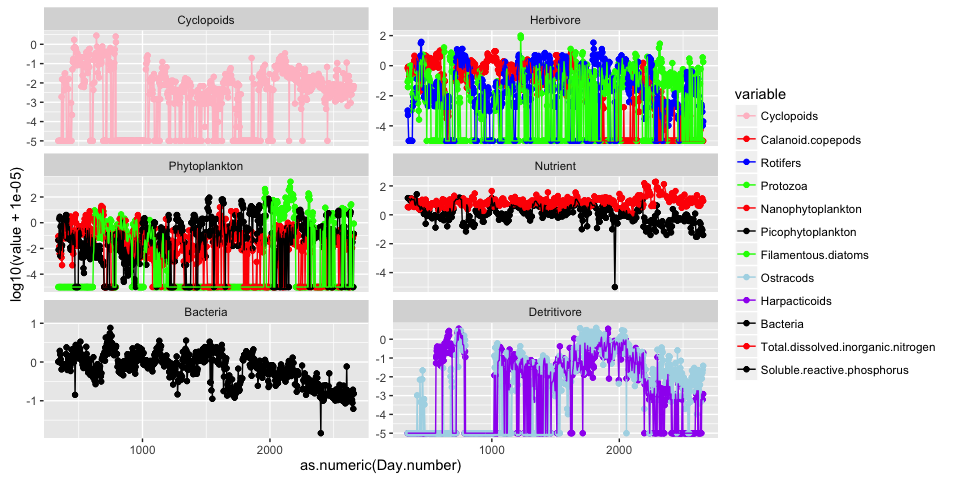
\includegraphics{figures/unnamed-chunk-21-1}
\caption{\label{fig:dynamics}Observed population dynamics.}
\end{figure}

\subsection{Data transformation}\label{data-transformation}

The following transformation steps were used:

\begin{enumerate}
\def\labelenumi{\arabic{enumi}.}
\tightlist
\item
  Time series shortened to remove long sequences of zeros.
\item
  Interpolation to create equally spaced observations in time series.
\item
  Fourth root transformation.
\item
  Detrending of five of the time series.
\item
  Rescaling to zero mean and unit standard deviation.
\end{enumerate}

The method for selecting the zeros to remove was unclear. In order to
reproduce this step, we removed the same data as in the original study,
by matching to the transformed data with zeros removed in the Ecology
Letters supplement Excel file mentioned above. All remaining
transformation steps were performed independently of this dataset. Our
reproduction of the transformed data closely matched the published
transformed data.

The data received directly from Stephen Ellner was interpolated, but
without zeros removed. Our interpolated data, without zeros removed,
matched closely this data.

\subsection{Correlations among species
abundances}\label{correlations-among-species-abundances}

Correlations among species abundances presented in Table 1 of the
original article closely matched our reproduced correlations, calculated
from the transformed data with zeros removed (figure
\ref{fig:corr_comp}). Deviations between the original and reproduced
correlations are relatively small (less than 0.072 units) and
infrequent. \textbf{These may have resulted from us removing zeros after
interpolation. Maybe we should check this.}

\begin{figure}[htbp]
\centering
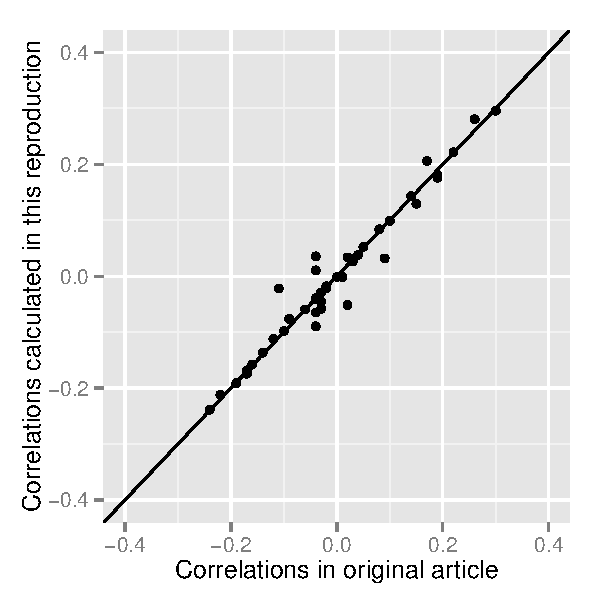
\includegraphics{figures/correlation_comparison.pdf}
\caption{\label{fig:corr_comp}Comparison of calculated correlations
among species abundances in the original article and this reproduction.}
\end{figure}

\subsection{Spectral analyses}\label{spectral-analyses}

\subsection{Lyapunov exponents by direct
method}\label{lyapunov-exponents-by-direct-method}

\subsection{Lyapunov exponents by indirect
method}\label{lyapunov-exponents-by-indirect-method}

\subsection{Predictability decay}\label{predictability-decay}

Only done for non-linear models (the original article also does this for
linear models).

\section{Conclusion}\label{conclusion}

Conclusion, at the very minimum, should indicate very clearly if you
were able to replicate original results. If it was not possible but you
found the reason why (error in the original results), you should exlain
it.

\begin{longtable}[c]{@{}llllll@{}}
\caption{\label{tbl:table}Table caption }\tabularnewline
\toprule
Heading 1 & & & Heading 2 & &\tabularnewline
\midrule
\endfirsthead
\toprule
Heading 1 & & & Heading 2 & &\tabularnewline
\midrule
\endhead
cell1 row1 & cell2 row 1 & cell3 row 1 & cell4 row 1 & cell5 row 1 &
cell6 row 1\tabularnewline
cell1 row2 & cell2 row 2 & cell3 row 2 & cell4 row 2 & cell5 row 2 &
cell6 row 2\tabularnewline
cell1 row3 & cell2 row 3 & cell3 row 3 & cell4 row 3 & cell5 row 3 &
cell6 row 3\tabularnewline
\bottomrule
\end{longtable}

A reference to table \ref{tbl:table}. A reference to figure
\ref{fig:logo}. A reference to equation \ref{eq:1}. A reference to
citation \textcite{markdown}.

\begin{figure}[htbp]
\centering
\includegraphics{rescience-logo.pdf}
\caption{\label{fig:logo}Figure caption}
\end{figure}

\begin{equation} A = \sqrt{\frac{B}{C}} \label{eq:1}\end{equation}

\section{Acknowledgements}\label{acknowledgements}

This reproduction was made as part of the Reproducible Research in
Ecology, Evolution, Behaviour, and Environmental Studies (RREEBES)
Course, lead by Owen Petchey at the University of Zurich. More
information about the course
\href{https://github.com/opetchey/RREEBES/blob/master/README.md}{here}
on github.

{\sffamily \small
  \printbibliography[title=References]
}
\end{document}
